\chapter{Project Phases}

This chapter describes the project phases used in the development of SitaWare Civilian.

Figure \ref{fig:project_phases} shows the six phases through which the system is to be developed. Furthermore, the figure contains the deliverables for the phase specific reviews. 

\begin{figure}[H]
\centering
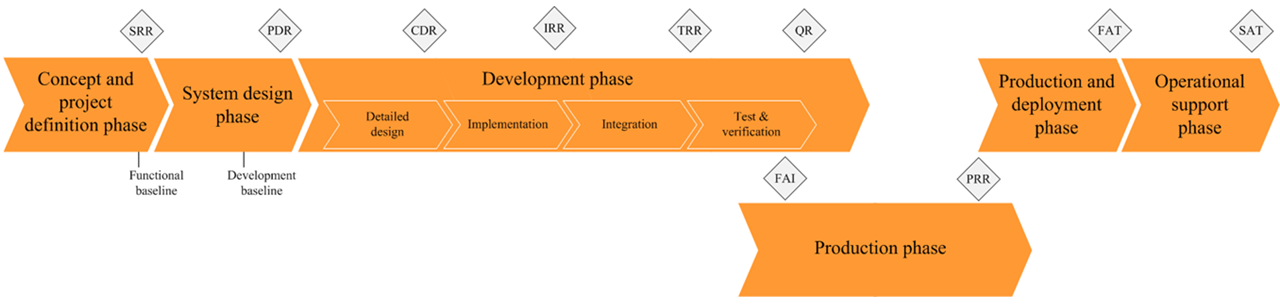
\includegraphics[width=0.95\textwidth]
{Billeder/project_phases/project_phases.PNG}
\caption{Project phases.}
\label{fig:project_phases}
\end{figure}


\paragraph{Concept and project definition phase}
This is the initial phase of the project and defines the problems and needs presented by the customer. By inspecting the needs, requirements to the system are identified. Furthermore, test methods for the defined requirements are specified. The phase ends with a system requirement review(SRR). 

Deliverables:
\begin{enumerate}
\item[•] Time plan
\item[•] System Requirement Specification(SRS)
\item[•] Concept of Operations(CONOPS)
\item[•] Traceability matrix
\end{enumerate}

\paragraph{System design phase}
In this phase the plan for the conduct of the project is created. The plan covers what and by whom and when the different project elements are carried out. 

\paragraph{Development phase}

\paragraph{Production phase}

\paragraph{Production and deployment phase}

\paragraph{Operational support phase}
